\section{Zeitplanung}
Die Initiale Zeitplanung wurde in jedem Iterationmeeting besprochen und entsprechend nachgeführt. Nachfolgend ist die Entwicklung der Planung zu sehen. Diese Nachführung hat den Zweck allfällige Abweichungen frühzeitig zu erkennen und entsprechend schnell reagieren zu können. Wöchentliche Iterationsmeetings im Entwicklungsteam intern und wöchentliche Statusmeetings mit Herrn Steffen \& Brunner stellen sicher, allfällig auftretende Komplikationen frühzeit zu erkennen.


\section{Iteration 0 / 1}
Die Primären Ziele der Iterationen 0 und 1 waren:
\begin{itemize}
\item Einlesen in die Thematik (Vorgänger BA cygnet / Aufgabenstellung / ISO Draft 19770-2)
\item Konfiguration der Entwicklungsumgebungen (IDE, Coding Guidelines, CI Travis, Github)
\item Definition Entwicklungsprozess, Projektmanagement-Methodik
\end{itemize}

\section{Iteration 2}
\subsection{Zeitplanung}
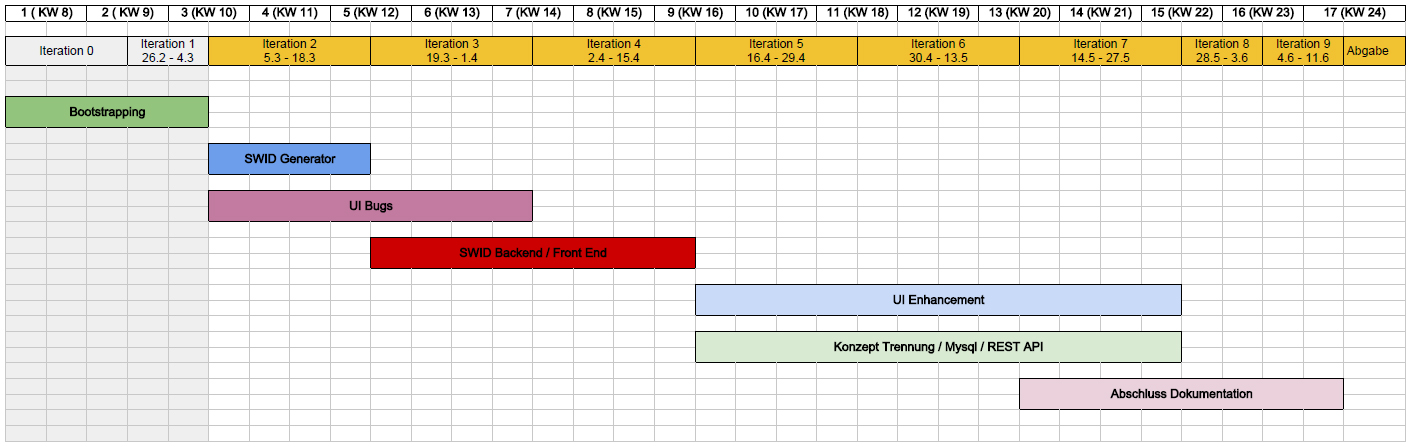
\includegraphics[scale=0.3]{images/zeitplanung/Iteration1_2.jpg}
\subsection{Meeting 3 5.3.2014}
\paragraph{Status}
Eine initiale Planung wurde erstellt. Die Planung ist so ausgelegt, das als erstes die Pflichtteile erarbeitet werden sollen. Einerseits zur Risikominierung für uns und andererseits soll dadruch sichergestellt sein, dass die geforderte Funktionalität,  die Herr Steffen im Juni demonstrieren will, möglichst bald fertig ist und danach ausgiebig getestet werden kann und bis zur Präsentation einen möglichst stabilen Stand erreicht. Sobald diese Funktionalitäten erreicht sind, werden die optionalen Teile in einem separaten Fork integriert um die Stabilität weiterhin zu gewährleisten.
Das SQLite Schema wurde testweise auf MySql/Maria DB portiert. Dabei wurden einige Probleme festgestellt:
\begin{itemize}
\item Tabellennamen sowie Felder verwenden MySql Keywords wie Key/Keys
\item Es gibt Indizes über Felder des Types TEXT, das ist in Mysql so nicht möglich, eine einschränkung über deren länge ist nötig.
\item Die Referenzen in SQLite Syntax sind nur zur dokumentation vorhanden, sind aber leider etwas fehlerhaft. Es gibt verweise auf die nicht existente Tabelle measurements und einige Referenzen fehlen ganz. 
\end{itemize}

\paragraph{Zusammenfassung}

\begin{itemize}
\item Pflichtteile werden in der Planung priorisiert.
\item Die Migration auf MySQL wird nach hinten geschoben, da nicht pflicht und einige Probleme daraus resultieren könnten
\item
\end{itemize}
\subsection{Meeting 4 12.3.2014}
\paragraph{Status}
Der Zeitplan konnte bisher eingehalten werden. Der Stand des SWID Generators konnte im Meeting vorgeführt werden, sieht soweit gut aus. 
Die File Tags sollen optional im output enthalten sein, um das Mapping von Files und Pakete zu erhalten. Dazu gibt es einen Use Case welchen wir im Frontend auch berücksichtigen sollten, siehe Todo. Wir haben noch lange über das Sequenzdiagramm diskutiert, es gibt es da noch einige Zuständigkeiten der einzelnen Komponenten, die noch nicht ganz klar sind. Wir werden das nächste Meeting das überarbeitete Diagramm nochmals mitbringen.

\paragraph{Zusammenfassung}
\begin{itemize}
\item Parameter für xml dokument separator (default: 2x newline)
\item Use gibt einen UseCase: File Hash stimmt nicht, aus welchem Pakage kommt das file?
\item Autodetection des Environments (dpkg/yum)
\item Deployment soll als executable vorliegen, dass zb mittels pip installiert werden kann
\item Nur installierte Packages auflisten, ist momentan noch nicht implementiert
\end{itemize}

\section{Iteration 3}
\subsection{Zeitplanung}
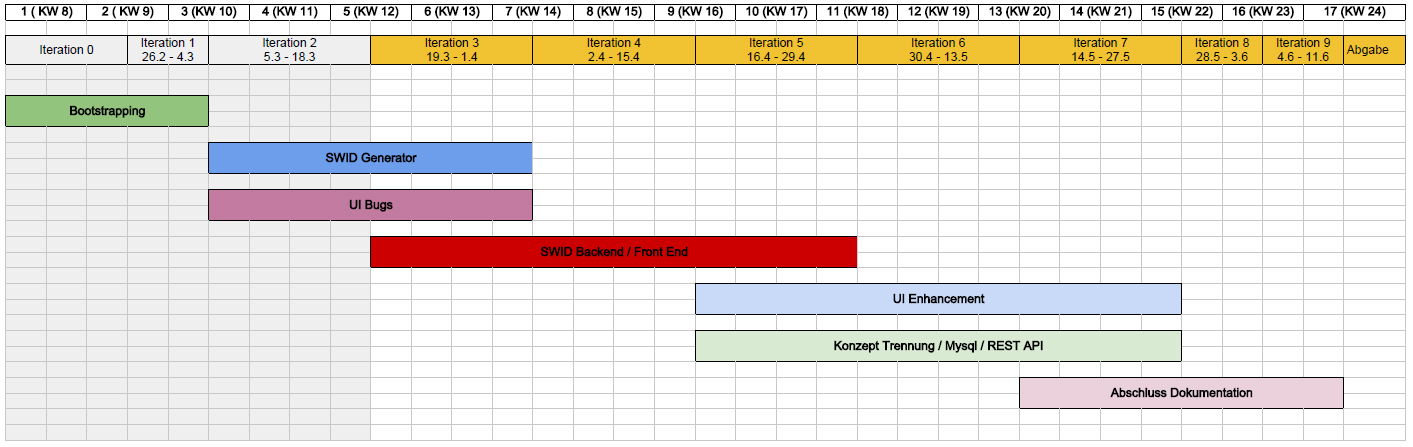
\includegraphics[scale=0.3]{images/zeitplanung/Iteration3.jpg}
\subsection{Meeting 19.3.2014}
\paragraph{Status}

Wir liegen nicht ganz im Zeitplan, da Danilo zur Zeit noch im Spital ist. Entsprechend haben wir den Zeitplan angepasst und die Ziele etwas nach hinten in den vorgesehenen Puffer verschoben. Bis auf das File Listing konnten wir in dieser Iteration alle Ziele erreichen. Wir haben am Meeting eine erste Version des Datenmodells für die SWID Tag vorgestellt. Es gabe da einige Diskussionspunkte. Zum einen stellte sich die Frage ob wir die Daten in das bestehende Modell integrieren sollen oder komplett als Erweiterung (separate Tabellen). Folgende Punkte sind in der Diskussion aufgefallen
\begin{itemize}
\item XML String sollte RAW auch abgespeichert werden

\paragraph{Zusammenfassung}
\begin{itemize}
\item Readme für die SWID Generator Installation erstellen
\item Die Anforderungen ans Backend sind noch nicht sehr klar, wir beginnen mit erfassen von Use Cases, damit könnten sich viele Fragen zum Datenmodell beantworten lassen.
\item Blacklist Option im Package View ist überflüssig
\item Pull Request von aktuellem Stand (strongTNC) erstellen
\item Beim UI sollte bei der Suche bzw. Autocomplete auch die Option angeboten werden ein neues Item zu erstellen -> Usability
\end{itemize}
\end{itemize}

